\chapter{Farmaci delle patologie del SN}

\section{Farmaci sedativo/ansioliti e ipnotici}

Classificazione sulla base dell'utilizzo clinico e non già sulle struttura chimica in quanto molto variabile

\begin{tikzpicture}
	\Tree
	[.{scopo}
		[.\node(sedazione){sedazione};
			[.{ansiolitico\\ (\dwa stato ansia)}
				[.tranquillante
					\node(aum){aumentando dosaggio};
				]
			]
		]
		[.\node(ipnotico){ipnotico};
			[.{sonnolenza\\ (\upa sonno)}
				\node(dep){depressione SN maggiore};
			]
		]
	]
	\draw[drawarrow] (aum) to[out=-145,in=-20] (ipnotico);
	\draw[drawarrow] (dep) to[out=0,in=20] (sedazione);
\end{tikzpicture}

\begin{tikzpicture}
	\Tree
	[.{relazione \\ dose/risposta\\ lineare}
		[.sedazione
			[.ipnotico
				[.anestesia
				]
			]
		]
	]
	\begin{scope}[yshift=-3em,xshift=3em]
	\Tree
	[.\node[dummyc]{};
		[.{depressione centri\\ respiro}
			[.coma
				morte
			]
		]
	]
	\end{scope}
\end{tikzpicture}

{grafico}

Quelli più nuovi richiedono dosi non--lineari per le fasi post--ipnotich

\begin{tikzpicture}
	\tikzset{level 1/.style={level distance=130pt}}
	\tikzset{frontier/.style={distance from root=250pt}}
	\Tree
	[.{tipologie}
		[.benzodiazepine
			\node[farmaco]{\index{diazepam}diazepam\\ emivita $12\sim72$h\\(valium - ansiol.)};
			\node[farmaco]{\index{lorazepam}lorazepam\\ emivita $2\sim6$h\\(tavor - ansiol.)};
			\node[farmaco]{\index{flunitrazepam}flunitrazepam\\ emivita $8\sim24$h\\(roipnol - ansiol./ipnot.)};
		]
		[.barbiturici
			\node[farmaco]{\index{pentobarbital}pentobarbital\\(ipnotico)};
			\node[farmaco]{\index{fenobarbital}fenobarbital\\(ipnotico)\\(più come antiepilettico)};
			\node[farmaco]{\index{tiopental}tiopental\\(ipnotico)\\(più come anestetico generale\\ siero della verità)};
		]
		\node[farmaco]{\index{buspirone}buspirone\\ (ansiol.)};
		[.{ipnotici\\ non benzodiazepinici}
			\node[farmaco]{\index{zolpidem}zolpidem};
			\node[farmaco]{\index{zaleplon}zaleplon};
		]
		[.antipsicotici
			\node[farmaco]{\index{ATC}ATC\\(vedi sezione)};
		]
		[.antidepressivi
			{i più recenti SSRI e SNRI\\ (vedi sezione)}
		]
		[.antiepilettici
			\node[farmaco]{\index{valproato}valproato\\(vedi sezione)\\(ansiol.)};
		]
	]
\end{tikzpicture}

\begin{tikzpicture}
	\Tree
	[.{Effetti BZD,\\ barbiturici e non}
		sedazione
		ipnosi
		{anestesia\\ (vedi dopo)}
		{anticonvulsivi\\ (vedi sezione)}
		{miorilassanti\\ (non i più recenti)}
		{depressione respiro\\ (soprattuto se già depresso\\ per altre patologie)}
	]
\end{tikzpicture}



\begin{tikzpicture}
	\Tree
	[.{bezodiazepine}
		[.meccanismo
			[.{recettore \ce{GABA_a}\\ nel sito BZ}
				[.{isoforma\\ con subunità $\alpha_1$}
					{effetto sedativo/ipnotico}
				]
				[.{con subunità $\alpha_2$}
					{effetto solo sedativo}
				]
			]
		]
		[.assunzione
			os EV
		]
		[.metabolismo
			[.epatico
				[.{lunga emivita}
					{desmetilazione (desmetildiazepam)\\ con formazione\\ metabolita attivo\\ con emivita $>40$h}
				]
				[.{breve emivita}
					[.{glucuronazione e\\ escrezione renale\\ solo \index{diazepam}diazepam}
					]
				]
			]
		]
		[.emivita
			{$\sim$ 1h per \upa clearenace epatica}
		]
		[.{effetti terapeutici}
			{$\downarrow$ansia\\ $\downarrow$aggressicità\\ induzione sonno}
		]
		[.{effetti collaterali}
			{amnesia anterograda\footnotemark\\ tolleranza ($\uparrow$dose)\\ dipendenza psicofisica\\ depressione sistema respiratorio }
		]
	]
\end{tikzpicture}

\footnotetext{Incapacità a ricordare azioni avvenute durante l'azione del farmaco. Roipnol, la droga dello stupro.}

Per anatagonizzare i sovradosaggi delle benzodiazepine si usa il flumazenil, anche lui una benzodiazepina ma con azione antagonista su BZ.

Alcune BZD come diazepam, lorazepam sono usati IV nell'induzione dell'anestesia con probabile contributo della depressione respiratoria post--anestesia.

\begin{tikzpicture}
	\Tree
	[.{flumazenil}
		[.{antagonista\\ recettore BZ}
			[.{blocca l'azione di}
				benzodiazepine
				{non--benzodiazepine}
			]
			[.{non blocca l'azione di}
				barbiturici
				etanolo
			]
		]
	]
\end{tikzpicture}

\begin{tikzpicture}
	\Tree
	[.\node[farmaco]{\index{buspirone}buspirone\\(non in Italia)};
		[.meccanismo
			{agonista parziale \ce{5-HT_{1A}} e \ce{D_2}}
		]
		[.assunzione os
		]
		[.metabolismo epatico
		]
		[.{effetti terapeutici}
			[.vantaggi
				{ansiolitico\\ no sedazione\\ no dipendenza\\ no ansia da interruzione}
			]
			[.svantaggi
				{necessario settimane prima\\ che inizino gli effetti}
			]
		]
		[.{effetti collaterali}
			{nausea\\ vertigini\\ irrequietezza}
		]
	]
\end{tikzpicture}

\begin{tikzpicture}
	\Tree
	[.barbiturici
		[.meccanismo
			{recettore \ce{GABA_a}\\ in sito differente da BZ}
		]
		[.assunzione {os,EV}
		]
		[.metabolismo epatico
		]
		[.{effetti terapeutici}
			{depressione non selettiva del SNC\\ attualmente usati come\\
			antiepilettici e anestetici
			}
		]
		[.{effetti collaterali}
			{alta tolleranza\\ alta dipendenza\\ induttori P450\\ depressione cardiopolmonare}
		]
	]
\end{tikzpicture}

\begin{tikzpicture}
	\tikzset{level 1/.style={level distance=130pt}}
	\Tree
	[.{ipnotici non--benzodiazepinici}
		[.meccanismo
			[.{recettore \ce{GABA_a}\\ con sole unità $\alpha_1$}
				{sedazione ma non ansiolitico}
			]
		]
		[.assunzione {os}
		]
		[.metabolismo epatico
		]
		[.{effetti terapeutici}
			{trattamento insonnia\\ no tolleranza\\ no dipendenza
			}
		]
		[.{effetti collaterali}
			{interferenza con alcol\\ depressione SNC ad alte dosi}
		]
	]
\end{tikzpicture}

\begin{tikzpicture}
	\Tree
	[.{qualità sonno}
		{1. latenza prima inizio sonno}
		{2. fase non--REM (NREM)}
		{3. fase REM}
		{4. fase NREM a onde lente}
	]
	\begin{scope}[xshift=14em]
		\node(par){$\left.\rule{0pt}{46pt}\right\}$};
		\node[text width=10em] at (2.5,0){ideale $\downarrow$1. $\uparrow$2. $\uparrow$3. $\uparrow$4. };
	\end{scope}
\end{tikzpicture}

\begin{tikzpicture}
	\Tree
	[.{effetto farmaci\\ sul sonno}
		[.benzodiazepine
			{$\downarrow$1. $\uparrow$2. $\downarrow$3. $\downarrow$4. }
		]
		[.{non--benzodiazepine}
			{$\downarrow$1. ininfluente sugli altri }
		]
	]
\end{tikzpicture}

Tutti questi farmaci si legano al \ce{GABA_A} tranne il buspirone che agisce come agonista parziale per \ce{5-HT_{1A}} e \ce{D_2}.

\ce{GABA_B} attivato da agenti spasmolitici come baclofene.

Tutti \upa inibizione GABAergica \upa permeabilità al \ce{Cl-} del canale \ce{GABA_A} tramie interazione allosterica con GABA.

\begin{tikzpicture}
	\Tree
	[.{apertura canale}
		[.benzodiazepine
			{\upa frequenza apertura}
		]
		[.barbiturici
			{\upa durata apertura}
		]
	]
\end{tikzpicture}

I barbiturici sono anche GABA--mimetici quindi funzionano teoricamente anche senza GABA.

\section{Farmaci anti--psicotici}

La schizzofrenia è una persistente alienazione del pensiero che da sia disturbi positivi, con caratteristiche psicologiche aggiunte quali delirio, allucinazioni e aggressività, sia sintomi negativi, con caratteristiche psicologiche perse quali isolamento sociale, apatia e mancanza di iniziativa.

Le teorie fisiopatologiche di questo disturbo sono tre. Una teoria dopaminergica che spiega i sintomi positivi che deriva la patologia da una iperstimolazione dei recettori~\ce{D_2}/\ce{D_4}; una teoria glutammatergica che deriva la patologi da bassi livelli di glutammato e da una conseguente iperstimolazione del recettore~NMDAM; una teoria serotoninergica derivata dall'osservazione che gli antagonisti serotoninergici sono antipsicotici e che l'LSD, un agonista~5-HT, fa venire i sintomi positivi.

I farmaci usati si dividono in tipici a atipici. I tipici quali i fenotiazidici come la \index{clorpromazina}clorpromazina e i butirrofenonici come l'\index{aloperidolo}aloperidolo (Serenase), agiscono bloccando i recettori dopaminergici diminuendo i sintomi positivi e, i più recenti, anche quelli negativi ma hanno effetti collaterali sul sistema extrapiramidale come distonie acute e tardive. 

Gli atipici non hanno effetti sulla via extrapiramidale in quando bloccano selettivamente la via mesolimbica (della gratificazione) ignorando la via nigrostriata e sono quindi usati principalmente se gli effetti collaterali dei tipici sono eccessivi. Tali farmaci bloccano anche i recettori $\alpha$--adrenergici e i~5-HT e sono la \index{clorapina}clorapina (una dibenzodiazepina) e l'\index{olanzapina}olanzapina.

Il difetto di tutti i farmaci anti--psicotici descritti è che impiegano settimane prima del loro effetto terapeutico e questo è un segno che vi deve essere un qualche altro effetto secondario ad agire come, ad esempio, l'aumento dei~\ce{D_2} a livello limbico.

\begin{tikzpicture}
	\tikzset{level distance=150pt}
	\Tree
	[.{schizzofrenia}
		{persistenza di alterazioni del pensiero,\\ del comportamente e delle affettività}
	]
\end{tikzpicture}

\begin{tikzpicture}
	\Tree
	[.{sintomi}
		[.{positivi\\(caratt. psicol. aggiuntive)}
			delirio
			allucinazioni
			{pensieri disorganizzati}
			aggressività
			{convinzioni errate}
		]
		[.{negativi\\(caratt. psicol. perse)}
			{isolamento sociale}
			apatia
			{mancanza di iniziativa}
			{insensibilità emotiva}
		]
	]
\end{tikzpicture}

\begin{tikzpicture}
	\tikzset{level distance=80pt}
	\Tree
	[.{fisiopatologia}
		[.positivi
			[.{inibizione GABAesrgica\\ \ce{D_2} mediata}
				inibizione
			]
		]
		[.negativi
			[.{\dwa n. di recettori \ce{D_1}}
				[.{iperattività GABA}
					[.{inibizione\\ glutammatergica}
						{ipostimolazione del\\ recettore NMDA}
					]
				]
			]
		]
	]
\end{tikzpicture}

\begin{tikzpicture}
	\Tree
	[.{teorie fisiopatologiche}
		[.{teoria dopaminergica\\ (in disuso)}
			[.{spiega sintomi positivi\\ perchè i farmaci dopaminergici\\ causano psicosi}
				{\upa stimolazione \ce{D_2}/\ce{D_4}\\ oppure \upa stim. \ce{D_2}, \dwa stim. \ce{D_4}\\ pazienti schizzofrenici hanno \\\upa densità \ce{D_2} e \upa dopamina}
			]
		]
		[.{teoria glutammatergica}
			[.{bassi livelli\\ di glutammato}
				[.{spiega sintomi negativi}
					{\dwa stimolazione NMDA\\ perchè farmaci di questo tipi\\ causano carenze psichice}
				]
			]
		]
		[.{teoria serotoninergica}
			[.{sintomi negativi}
				{antagonisti serotoninergici\\ sono anti--psicotici}
			]
			[.{sinitomi positivi}
				{LSD (agonista 5-HT) fa\\ venire i sintomi positivi}
			]
		]
	]
\end{tikzpicture}

\begin{definizione}{EPS} 
Effetti collaterali extrapiramidali, catalessi nelle cavie
\end{definizione}
 

\begin{definizione}{Agente neurolettico}
alta incidenza di EPS a dosi efficaci
\end{definizione}

\begin{tikzpicture}
	\tikzset{frontier/.style={distance from root=300pt}}
	\Tree
	[.{farmaci}
		[.{tipici\\ (hanno effetti neurolettici)}
			[.fenotiazidici
				\node[farmaco]{\index{clorpromazina}clorpromazina\\ agente neurolettico};
			]
			[.butirrofenonico
				\node[farmaco]{\index{aloperidolo}aloperidolo\\ (serenase)};
			]
		]
		[.{atipici\\ (non hanno effetti neurolettici)}
			\node[farmaco]{\index{clozapina}clozapina\\(dibenzodiazepina)};
			\node[farmaco]{\index{olanzapina}olanzapina};
		]
	]
\end{tikzpicture}

La \index{reserpina}reserpina, ora in disuso, ha effetti collaterali di tipo parkinsoniano con blocco sistema dopaminergico

I farmaci anti--psicotici impiegano settimane per l'effetto, segno che vi sia un effetto secondario tipo incremento dei recettori \ce{D_2} a livello limbico.

Tutti hanno effetti a lunga durata (mesi) dopo l'ultima somministrazione. Solo \index{clozapina}clozapina non va mai sospesa bruscamente sie per le recidive rapide sia per effetti sfavorevoli quali miocarditi e agranulocitosi.

\begin{tikzpicture}
	\tikzset{level 2/.style={level distance=150pt}}
	\Tree
	[.{tipici}
		[.meccanismo
			{blocco recettori \ce{D_1}/\ce{D_2}}
		]
		[.assorbimento
			{os, intramuscolo}
		]
		[.metabolismo
			{epatico via cit. P450\\ isoforme CYP2D6, CYP1A2/A4\\ escrezione renale}
		]
		[.{usi clinici}
			{schizzofrenia: \dwa sintomi positivi\\ i più recenti anche \dwa sintomi negativi\\ anti--emetici}
		]
		[.{effetti collaterali}
			{EPS con distonia acuta\\ nelle prime settimane reversibili.\\ Discinesia tardiva con movimento\\ involontario di volto e lingua\\ causati da \upa n. \ce{D_2}}
		]
	]
\end{tikzpicture}

\begin{tikzpicture}
	\Tree
	[.{atipici}
		[.meccanismo
			{blocco \ce{D_2}, blocco $\alpha$--adrenergico\\ blocco 5--HT e \ce{D_4}\\ blocco recettori muscarinici}
		]
		[.assorbimento
			{intrauscolo}
		]
		[.metabolismo
			{epatico}
		]
		[.{effetti collaterali}
			{aumento di peso,\\ secchezza fauci,\\ stipsi,\\ ritenzione idrica,\\ ipotensione posturale\\ leucopenia}
		]
	]
\end{tikzpicture}

I farmaci atipici danno meno effetti collaterali motori perchè bloccano selettivamente la via mesolimbica (della gratificazione) invece del nigro--striato. Impegnati quindi se i sintomi extrapiramidali dei tipici fossero problematici.

\section{Farmaci antidepressivi}

\begin{tikzpicture}
	\tikzset{frontier/.style={distance from root=330pt}}
	\Tree
	[.{depressione}
		[.{disturbo dell'umore}
			[.{sintomi emozionali}
				{malessere, apatia, pessimismo}
				{bassa autostima}
				{incapacità a prendere decisioni}
				{idee di autolesionismo o\\ suicide}
			]
			[.{sintomi biologici}
				{ritardi nel pensiero o\\ nell'azione}
				{perdita di libibo}
				insonnia
				{perdita di appetito}
			]
		]
		[.{ma usati anche per}
			{attacchi panico}
			{disturbo d'ansia generalizzato}
			{disturbo post--traumatico da stress}
			{disturbo ossessivo compulsivo}
			{trattamento dolore neuropatico}
			{fibromialgia}
			{sindrome disforica pre--metruale}
		]
	]
\end{tikzpicture}


\begin{tikzpicture}
	\tikzset{level distance=90pt}
	\Tree
	[.{depressione}
		[.unipolare
			{variazioni di umore\\ sempre nello stesso verso}
		]
		[.{bipolare\\(sindrome maniaco\\ depressiva)}
			[.\node(d){depressione};
				[.\node(m){mania};
					\node(es){esuberanza};
				]
			]
		]
	]
	\node[below of=es,chartnode](e){entusiasmo};
	\node[below of=m,chartnode](im){impazienza};
	\node[below of=d,chartnode](c){collera};
	\draw[drawarrow] (es) -- (e) (e)--(im) (im)--(c) (c)--(d);
\end{tikzpicture}

\begin{definizione}{BDNF}
Brain--derivated neurotrophic factor: fattore di crescita nervoso
\end{definizione}


\begin{tikzpicture}
	\Tree
	[.{teorie\\ fisiopatologiche}
		[.{teoria monoaminergica\\ (vecchia)}
			[.\node[farmaco]{\dwa\index{noradrenalina}noradrenalina\\\dwa\index{serotonina}serotonina\dwa\index{dopamina}dopamina};
				[.\upa depressione ]
				[.\dwa {elevazione dell'umore} ]
			]
		]
		[.{teoria neutrofica\\ (più accreditata)}
			[.{perdita di neuroni e\\ di glia in ippocampo e\\ corteccia pre--frontale}
				[.depressione
					{\index{BDNF}BDNF porta a\\ elevazione dell'umore}
				]
			]
		]
	]
\end{tikzpicture}


\begin{tikzpicture}
	\Tree
	[.{teoria monaminergica}
		[.{\index{noradrenalina}noradrenalina, \index{serotonina}serotonina\\ innervano neuroni ipotalamici\\ che controllano\\ $\ominus$ l'ipofisi}
			[.{\upa CRH}
				[.{\upa ADCH}
					{\upa cortisolo\\(ormone dello stress)}
				]
			]
		]
	]
\end{tikzpicture}

\begin{tikzpicture}
\tikzset{frontier/.style={distance from root=400pt}}
	\Tree
	[.{farmaci}
		[.{inibitori\\ della ricaptazione}
			[.{della serotonina\\ blocco recettore SERT}
				[.SSRI
					\node[farmaco]{\index{fluoxetina}fluoxetina\\(prozac)};
				]
			]
			[.{della serotonina e\\ noradrenalina\\ blocco recettore NET}
				[.SNRI
					\node[farmaco]{\index{venlafaxina}venlafaxina};
				]
				[.{ATC\\(antidepressivi triciclici)}
					\node[farmaco]{\index{amitriptilina}amitriptilina};
					\node[farmaco]{\index{imipramina}imipramina};
				]
			]
		]
		[.{inibitori\\ delle monoamminossidasi\\(IMAO)}
			\node[farmaco]{\index{fenelzina}fenelzina\\(ritirato in Italia)};
			\node[farmaco]{\index{moclobemide}moclobemide};
		]
	]
\end{tikzpicture}

\begin{tikzpicture}
	\Tree
	[.{SSRI}
		[.meccanismo
			{\upa serotonina per\\ inibizione della ricaptazione}
		]
		[.assorbimento
			{os}
		]
		[.metabolismo
			[.{passa per \index{norfluoxetina}norfluoxetina,\\ composto attivo con\\ emivita 3x fluoxetina}
				{epatico con interazione con\\ ATC, CYP2D6}
			]
		]
		[.{usi clinici}
			{depressione, ansia, \\ panico,\\ disordine ossessivo--compulsivo}
		]
		[.{effetti collaterali}
			{nausea, vomito, insonnia,\\ sindrome serotoninergica (tremore\\ collasso cardiocirc., ipertermia)}
			{4 settimane di interruzione\\ prima di usaun un IMAO}
		]
	]
\end{tikzpicture}

\begin{tikzpicture}
	\Tree
	[.{ATC}
		[.meccanismo
			{\upa serotonina per\\ inibizione della ricaptazione}
			{noradrenalina per competizione\\ con i siti di legame}
		]
		[.assorbimento
			{os}
		]
		[.metabolismo
			{epatico con grande volume\\ di distribuzione e lento\\ metabolismo e quindi\\ stretta finestra terapeutica}
		]
		[.{usi clinici}
			{panico, antidepressivo, \\ analgesico nella cura\\ del dolore neuropatico}
		]
		[.{effetti collaterali}
			{atropina--like,\\ ipotensione posturale,aritmie\\ depressione respiratoria\\ con alcol}
			{ATC + IMAO MAI per rischio\\ ipertensione acuta}
		]
	]
\end{tikzpicture}

Il 10\% dei caucasici ha una mutazione del gene della CYP2D6 con effetti collaterali agli ATC molto più pesanti

\begin{tikzpicture}
	\tikzset{level 2/.style={level distance=150pt}}
	\Tree
	[.{IMAO}
		[.meccanismo
			[.{vecchi farmaci\\(fenelzina)}
				{inibizione irreversibile\\ dell'enzima MAO.\\ }
			]
			[.{nuovi farmaci\\(moclobemide)}
				{inibizione reversibile\\ dell'enzima MAO.\\ }
			]
		]
		[.{usi clinici}
			{\upa conc. plasm. 5-HT, \ce{Na+} e dopamina\\ Euforia e eccitazione}
		]
		[.{effetti collaterali}
			{ipotensione caratteristica per\\ dwa rilascio noradrenalina.}
			{downreg. recettori $\beta$--adrenergici e 5-HT}
			{cheese reaction con crisi ipertensiva acuta\\ perchè \index{tiramina}tiramina contenuta nei\\ formaggi non viene degradata\ dalle MAO inibite}
			{ATC + IMAO MAI per rischio ipertensione acuta}
		]
	]
\end{tikzpicture}

Di solito quindi la terapia è ATC + SSRI.

\begin{tikzpicture}
	\Tree
	[.{stabilizzazione\\ dell'umore}
		\node[farmaco]{\index{litio}litio};
		[.antiepilettici
			\node[farmaco]{\index{carbamazepina}carbamazepina};
			\node[farmaco]{\index{valproato}valproato};
		]
	]
\end{tikzpicture}


\begin{tikzpicture}
	\tikzset{level 2/.style={level distance=130pt}}
	\tikzset{level 3/.style={level distance=130pt}}
	\Tree
	[.{Litio}
		[.meccanismo
			[.{$\ominus$ inositolo monofosfato}
				{depressione cirtuiti iperattivi}
			]
			[.{$\ominus$ gliglogenosinetasi chinasi (GSK-3)}
				{attivazione enzimi apoptotici}
			]
			{\dwa cAMP}
		]
		[.assorbimento
			{os sotto forma di carbonato}
		]
		[.metabolismo
			[.{renale lenta\\ 1$\sim$2 settimane}	
				{stretta finestra terapeutica\\ pericolo sovradosaggio}
			]
		]
		[.{usi clinici}
			{profilassi e trattamento di\\ depressione uni e bipolare}
		]
		[.{effetti collaterali}
			{tremore (si riduce \\con \index{propranololo}propranololo)}			
			[.{+ diuretici}
				{\dwa \ce{Na+}}
			]
			{nausea, vomito, diarrea}
			[.{ritensione di \ce{Na+} e\\ \upa aldosterone}
				{danni tubulari}
			]
			{\dwa funzione tiroidea\\ e ipertiroidismo}
			{\upa peso corporeo e edema}
		]
	]
\end{tikzpicture}

Carbamazepina: $\ominus$ IP

Valproato: $\ominus$ IP + $\ominus$ GSK-3


\section{Farmaci antiepilettici}

\begin{tikzpicture}
	\tikzset{frontier/.style={distance from root=400pt}}
	\Tree
	[.{epilessie}
		[.parziali
			[.{inizio locus\\ encefalico specifico}
				[.{resta specifico}
					{semplice}
				]
				[.{si diffonde}
					{complesso}
				]
			]
			[.{evolve in grande male}
				{secondarie}
			]
		]
		{spasmi infantili\\(sindrome epilettica)}
		[.generalizzate
			{tonico--cloniche\\(grande male)}
			toniche
			{(mio)cloniche}
			{atoniche\\(perdita tono posturale)}
			{assenze\\(piccolo male)}
		]
	]
\end{tikzpicture}

\begin{tikzpicture}
	\tikzset{level distance=150pt}
	\Tree
	[.{farmaci}
		[.\node[farmaco](fenitoina){\index{fenitoina}fenitoina};
			\node(parziali){parziali};
		]
		[.\node[farmaco](carba){\index{carbamazepina}carbamazepina};
			\node(tc){tonico--cloniche};
		]
		[.\node[farmaco](val){\index{valproato}valproato};
			\node(assenze){assenze};
		]
		[.\node(benzo){benzodiazepine};
			\node(miocloniche){miocloniche};
		]
		[.\node[farmaco]{\index{etosuccimide}etosuccimide};
			\node(atoniche){atoniche};
		]
		[.\node[farmaco]{\index{corticotropina}corticotropina};
			\node(spasmi){spasmi infantili};
		]
		[.\node[farmaco]{\index{diazepam}diazepam\\ benzodiazepina + \\ fosfenitoina (simil\\ fenitoina ma IV o IM)};
			{emergenze epilettiche}
		]
		[.\node[farmaco]{\index{acetazolamide}acetazolamide\\(diuretico inibizione\\ anidrasi carbonica)}; tutti
		]
	]
	\draw[drawarrow] (fenitoina) to[out=0,in=180] (tc);
	\draw[drawarrow] (carba) to[out=0,in=180] (parziali);
	\draw[drawarrow] (val) to[out=0,in=180] (tc);
	\draw[drawarrow] (val) to[out=0,in=180] (miocloniche);
	\draw[drawarrow] (val) to[out=0,in=180] (atoniche);
	\draw[drawarrow] (benzo) to[out=0,in=180] (atoniche);
	\draw[drawarrow] (benzo) to[out=0,in=180] (spasmi);
\end{tikzpicture}

\begin{tikzpicture}
	\tikzset{level 2/.style={level distance=150pt}}
	\tikzset{level 3/.style={level distance=80pt}}
	\tikzset{level 4/.style={level distance=80pt}}
	\Tree
	[.\node[farmaco]{\index{fenitoina}fenitoina\\(più antico)};
		[.meccanismo
			[.{inibizione canali \ce{Na+}}
				[.{+$\uparrow$freq. scarica}
					{+$\uparrow$blocco}
				]
			]
		]
		[.assunzione {os, EV solo fosfenitoina}
		]
		[.metabolismo {epatico dose--dipendente fino a un limite\\ oltre il quale piccoli $\uparrow$dosi\\ producono grandi $\uparrow$conc. ematica}
		]
		[.{effetti terapeutici}
			{parziali e tonico--cloniche.\\ Non assenze che può causare
			}
		]
		[.{effetti collaterali}
			{induttore P450}
			{trasp. da albumina ma\\ \index{valproato}valproato ha maggiore affinità e\\ quindi causa $\uparrow$conc. farmaco libero}
			{vertigini, cefalee, nistagmo}
			{possibile effetto teratogeno}
		]
	]
\end{tikzpicture}

\begin{tikzpicture}
	\Tree
	[.\node[farmaco]{\index{{carbamazepina}}carbamazepina};
		[.meccanismo
			{come fenitoina + blocco \ce{Ca^2+}}
		]
		[.assunzione {os}
		]
		[.metabolismo ???
		]
		[.{effetti terapeutici}
			{tutti tranne assenze}
		]
		[.{effetti collaterali}
			[.{induttore P450}
				{accellera il\\ metabolismo della\\ fenitoina e warfarin}
			]
			[.{epossido}
				sonnolenza
				{ritenzione idrica}
				epatotossicità
			]
		]
	]
\end{tikzpicture}

\begin{tikzpicture}
	\tikzset{level 2/.style={level distance=150pt}}
	\Tree
	[.\node[farmaco]{\index{{valproato}}valproato};
		[.meccanismo
			[.{come fenitoina + inibizione\\ di due enzimi che inattivano\\ il GABA}
				{$\uparrow$GABA}
			]
		]
		[.assunzione {os}
		]
		[.metabolismo ???
		]
		[.{effetti terapeutici}
			{tonico--cloniche e assenze}
			{bassa tossicità}
			{no azione sedativa}
		]
		[.{effetti collaterali}
			{rari casi assottigliamento capelli}
			{rari casi teratogenicità\\ con spina bifida}
			{spiazza fenitoina\\ dalle proteine plasmatiche}
			[.{inibisce il metabolismo di}
				\node[farmaco]{\index{fenobarbital}fenobarbital};
				\node[farmaco]{\index{fenitoina}fenitoina};
				\node[farmaco]{\index{carbamazepina}carbamazepina};
			]
		]
	]
\end{tikzpicture}

\begin{tikzpicture}
	\tikzset{level 2/.style={level distance=150pt}}
	\Tree
	[.\node[farmaco]{\index{etosuccimide}etosuccimide};
		[.meccanismo
			[.{inibizione dei canali \ce{Ca^2+}\\ a bassa soglia}
				{responsabili delle correnti\\ corticali ritmiche\\ nelle assenze}
			]
		]
		[.assunzione {os}
		]
		[.metabolismo epatico
		]
		[.{effetti terapeutici}
			assenze
		]
		[.{effetti collaterali}
			{nausea\\ letargie\\ crisi tonico--cloniche}
		]
	]
\end{tikzpicture}

\begin{tikzpicture}
	\Tree
	[.{altri farmaci recenti}
		[.\node[farmaco]{\index{vigabatrin}vigabatrin};
			[.{si lega irreversibilmente\\ a GABA--amministranferasi}
				{$\uparrow$GABA nel cervello}
			]
		]
		[.\node[farmaco]{\index{lamotrigina}lamotrigina};
			{blocco \ce{Na+} per assenze}
		]
		[.\node[farmaco]{\index{felbamato}felbamato};
			{blocco uso--dipendente NMDA.\\ Si usa solo nelle epilessie\\ intrattabili a causa\\
			dei suoi effetti collaterali\\ (anemia aplastica e epatite)}
		]
	]
\end{tikzpicture}

\section{Malattia di Alzheimer (AD)}

\begin{tikzpicture}
	\Tree
	[.{AD}
		[.idiopatica
			{demenza per--senile}
		]
	]
\end{tikzpicture}

\begin{tikzpicture}
	\Tree
	[.{patogenesi}
		[.\node(a){perdita di neuroni\\ colinergici};
			ippocampo
			{corteccia frontale}
			{nuclei della base}
		]
		[.\node(b){presenza placche\\ amiloidi};
			[.{depositi intracellulari\\ di $\beta$--amiloidi (A$\beta$)}
				apoptosi
			]
		]
	]
	\draw[drawarrow] (b)--(a) node[midway, below, sloped,smallfont] {causa};
\end{tikzpicture}

\begin{tikzpicture}
	\tikzset{frontier/.style={distance from root=200pt}}
	\Tree
	[.{farmaci}
		[.{inibitori della\\ colinesterasi}
			\node[farmaco]{\index{tacrina}tacrina};
			\node[farmaco]{\index{rivastigmina}rivastigmina};
		]
		\node[farmaco]{\index{diidroergotamina}diidroergotamina};
		[.{antagonisti recettore\\ NMDA}
			\node[farmaco]{\index{memantina}memantina};
		]
	]
\end{tikzpicture}

\begin{tikzpicture}
	\Tree
	[.{inibitori della\\ colinesterasi}
		[.meccanismo
			{$\uparrow$trasmissione colinergica}
		]
		[.assorbimento os
		]
		[.metabolismo epatico
		]
		[.{usi clinici}
			{piccolo miglioramento\\ funzionalità}
			{no effetti su progressione\\ malattia}
		]
		[.{effetti collaterali}
			{nausea\\ crampi addominali\\ apatotossicità (tacrina)}
		]
	]
\end{tikzpicture}

\begin{tikzpicture}
	\Tree
	[.{antagonisti recettore\\ NMDA}
		[.meccanismo
			{\dwa eccitossicità da glutammato}
		]
		[.assorbimento os
		]
		[.metabolismo epatico
		]
		[.{usi clinici}
			{migliore memoria}
		]
		[.{effetti collaterali}
			{diarrea\\ insonnia\\ incontinenza}
		]
	]
\end{tikzpicture}

\begin{tikzpicture}
	\Tree
	[.{eccitossicità glutammato}
		[.{\upa glutammato}
			[.{\upa stimolaziona AMPA\\ con sblocco NMDA}
				[.{liberazione \ce{Ca^2+}}
					\node[dummyc]{};
				]
			]
		]
	]
	\begin{scope}[yshift=-3em,xshift=3em]
	\Tree
	[.\node[dummyc]{};
		[.{\upa rilascio glutammato}
			[.{attivazione proteasi\\ \index{calpaina}calpaina e lipasi}
				{produzione di \ce{NO}\\ nel cervello}
				{rilascio acido arachidonico}
			]
		]
	]
	\end{scope}
\end{tikzpicture}

\begin{tikzpicture}
	\Tree
	[.\node[farmaco]{\index{diidroergotamina}diidroergotamina};
		[.meccanismo
			{vasodilatazione celebrale}
		]
		[.assorbimento {os,EV}		
		]
		[.metabolismo epatico
		]
		[.{usi clinici}
			{trattamento generale della demenza\\ efficacia limitata}
		]
	]
\end{tikzpicture}

\begin{tikzpicture}
	\Tree
	[.{altri farmaci}
		[.{FANS}
			\node[farmaco]{\index{ibuprofene}ibuprofene};
			\node[farmaco]{\index{indometacina}indometacina};
		]
		[.{agenti chelanti}
			{A$\beta$ include \ce{Cu},\ce{Zn}}
		]
		{immunizzazione contro le A$\beta$}
	]
\end{tikzpicture}

Anche impianto di cellule ingegnerizzate per produrre il fattore di crescita dei neuroni (fattore neurotrofico derivato dal cervello \index{BDNF}BDNF).

\section{Malattia di Parkinson (PD)}

\begin{tikzpicture}
	\Tree
	[.{PD}
		[.{malattia neurodegenerativa\\ cronica}
			[.{via extrapiramidale}
				[.{\dwa DOPA}, 
					{\upa azione Ach,\\ noradrenalina,\\ 5-HT e GABA}
				]
			]
		]
	]
\end{tikzpicture}

\begin{tikzpicture}
	%\draw[step=.5,very thin,yellow] (-2,0) grid (6,3);
	\node at (-2,.5) {Normale};
	\node(a) at (0,1) {};
	\node(b) at (2,0) {};
	\node(c) at (3,0) {};
	\node(d) at (5,0) {};
	\fill[Burlywood1] (-1,1.5) rectangle (1,-.5);
	\node[smallfont] at (0,1.75) {substantia nigra};
	\fill[LemonChiffon3] (1.5,1.5) rectangle (5.5,-.5);
	\node[smallfont] at (3.5,1.75) {corpo striato};
	\draw[neurone,red] (a.center) -| (c) node[near start,above,smallfont,black] {dopamina};
	\draw[neurone,green] (b.center) -- (c) node[midway,below,smallfont,black] {Ach.};
	\draw[neurone] (c.center) -- (d) node[at end,below,smallfont,black] {GABA};
	\begin{scope}[yshift=-6em]
		\node at (-2,.5) {Parkinson};
		\node(a) at (0,1) {};
		\node(b) at (2,0) {};
		\node(c) at (3,0) {};
		\node(d) at (5,0) {};
		\fill[Burlywood1] (-1,1.5) rectangle (1,-.5);
		\fill[LemonChiffon3] (1.5,1.5) rectangle (5.5,-.5);
		\draw[neurone,red, dashed] (a.center) -| (c);
		\draw[neurone,green] (b.center) -- (c);
		\draw[neurone] (c.center) -- (d);
		\end{scope}
\end{tikzpicture}

\begin{tikzpicture}
	\Tree
	[.{patogenesi}
		[.farmacologica
			[.{farmaci \dwa dopamina}
				\node[farmaco]{\index{reserpina}reserpina};
			]
			[.{farmaci bloccano\\ recettori dopaminergici}
				\node[farmaco]{\index{clorpromazina}clorpromazina\\ (antipsicotico)};
			]
		]
		[.{eventi neurotossici}
			{erbicidi, tossine ambientali...}
		]
		[.{cause genetiche}
			[.{corpi di Lewy}
				[.{accumulo di $\alpha$--sinvdeina\\ che precipita}
					{accumulo di\\ dopamina alterata}
				]
			]
			{alterazioni di\\ una parkina}
		]
	]
\end{tikzpicture}

\begin{tikzpicture}
	\Tree
	[.{sintomi}
		{tremore a riposo (Ach.)}
		{rigidità muscolare}
		{ipocinesia con difficoltà a\\ iniziare movimento (\dwa DOPA)}
		{andatura strisciante}
		{demenza senile}
	]
\end{tikzpicture}

\begin{tikzpicture}
	\tikzset{frontier/.style={distance from root=200pt}}
	\Tree
	[.{farmaci}
		[.{inibitore selettivo\\ delle MAO}
			\node[farmaco]{\index{selegilina}selegilina};
		]
		[.{agonisti dei \ce{D_2}}
			\node[farmaco]{\index{bromocriptina}bromocriptina};
			\node[farmaco]{\index{pergolo}pergolo};
		]
		\node[farmaco]{\index{levodopa}levodopa (L-DOPA) + \index{carbidopa}carbidopa};
		\node[farmaco]{\index{amantadina}amantadina\\(antivirale)};
		[.{antagonisti dell'Ach.}
			\node[farmaco]{\index{atropina}atropina};
			\node[farmaco]{\index{scopolamina}scopolamina};
		]
	]
\end{tikzpicture}

La dopamina come farmaco per os o parenterale non attraversa la barriera emato--encefalica (BEE).

\begin{tikzpicture}
	\Tree
	[.{L-dopa}
		\edge node[smallfont,yshift=1.2em,xshift=3.5em]{nel sangue};
		[.decarbossilata
			[.{dopamina nel sangue}
				{non attraversa BEE}
			]
		]
		\edge node[smallfont,yshift=-1em,xshift=4em]{1\%};
		[.{attraversa BEE}
			[.decarbossilata
				{dopamina nel cervello}
			]
		]				
	]
\end{tikzpicture}

ma carbidopa inibisce la decarbossilasi e non attraversa la BEE quindi non inibisce la decarbossilasi nel cervello per cui

\begin{tikzpicture}
	\Tree
	[.{L-dopa}
		\edge node[smallfont,yshift=-.5em,xshift=4.3em]{10\%};
		[.{attraversa BEE}
			[.decarbossilata
				{dopamina nel cervello}
			]
		]				
	]
\end{tikzpicture}

\begin{tikzpicture}
	\Tree
	[.\node[farmaco]{\index{levodopa}levodopa (L-DOPA) +\\ \index{carbidopa}carbidopa};
		[.meccanismo
			{\upa dopamina nel cervello}
		]
		[.assorbimento
			os
		]
		[.metabolismo
			{inattivazione intestinale e renale}
		]
		[.{usi clinici}
			{migliore rigidità e ipocinesia\\ nel 20\% spariscono tutti i sintomi\\ effetto\dwa nel tempo}
		]
		[.{effetti collaterali}
			{coree}
			{fluttuazioni dello\\ stato patologico\\ effetto on-off}
			[.{nelle prime settimane}
				{nausee, vomito, tachicardia}
				{sindrome simil--schizzofreniche}
				{sospensione periodiche\\ (drug holidays)\\ aiuta a ridurre\\ gli effetti collaterali\\ ma non gli on-off}
			]
		]
	]
\end{tikzpicture}

\begin{tikzpicture}
	\Tree
	[.\ce{MAOI_b}
		[.meccanismo
			[.{inibizione MAO}
				{\upa dopamina}
				{\dwa on-off}
			]
		]
		[.assorbimento
			{os}
		]
		[.{usi clinici}
			{migliora effetto levodopa}
		]
		[.{effetti collaterali}
			{insonnia, discinesie}
			{NON usare con altri MAO!!!\\ rischio ipertensione elevata}
		]
	]
\end{tikzpicture}

\begin{tikzpicture}
	\Tree
	[.{Agonisti dei \ce{D_2}}
		[.meccanismo
			{\upa stimolazione \ce{D_2}}
		]
		[.assorbimento
			{os}
		]
		[.metabolismo
			{epatico}
		]
		[.{usi clinici}
			{effetto duraturo. Per pazienti che\\ non tollerano L--dopa o che\\ sono diventati refrattari}
		]
		[.{effetti collaterali}
			{nausea, anoressia\\ ipotensione, confusione, allucinazioni}
		]
	]
\end{tikzpicture}

\begin{tikzpicture}
	\Tree
	[.\node[farmaco]{\index{amantadina}amantadina};
		[.meccanismo
			{\upa sintesi e rilascio dopamina}
			{\dwa ricaptazione dopamina}
		]
		[.assorbimento
			{os}
		]
		[.{usi clinici}
			{migliora bradicinesia e\\ rigidità ma si diventa\\ velocemente refrattari}
		]
		[.{effetti collaterali}
			{simili a L--dopa + ritenzione\\ urinaria, edema periferico}
		]
	]
\end{tikzpicture}

\begin{tikzpicture}
	\Tree
	[.{antagonisti dell'Ach.}
		[.meccanismo
			{\dwa effetti colinergici	}
		]
		[.assorbimento
			{os, EV}
		]
		[.metabolismo
			{idrolisi}
		]
		[.{usi clinici}
			{migliorano la rigidità ed\\ il tremore ma non hanno effetti su\\ ipo e bradicinesia}
		]
		[.{effetti collaterali}
			{discinesie, sonnolenza\\ stato confusionale}
		]
	]
\end{tikzpicture}

\newpage